\subsubsection{Ports - Incoming}

\subsubsubsection{AuthenticationUseCase} \label{AuthenticationUseCase}
\begin{figure}[H]
    \centering
    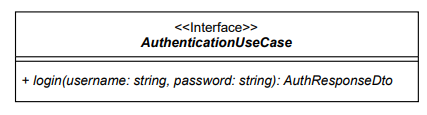
\includegraphics[width=0.65\textwidth]{assets/Backend/authentication_use_case.png}
    \caption{Diagramma dell'interfaccia AuthenticationUseCase}
  \end{figure}
\begin{itemize}
    \item \textbf{Descrizione}: AuthenticationUseCase definisce il contratto per i casi d'uso relativi all'autenticazione degli utenti;
    \item \textbf{Operazioni}:
    \begin{itemize}
        \item Autenticazione con username e password.
    \end{itemize}
    \item \textbf{Implementazione}: i dettagli dell'implementazione sono riportati nelle classi concrete.
\end{itemize}  

\subsubsubsection{DictionaryUseCase} \label{DictionaryUseCase}
\begin{figure}[H]
    \centering
    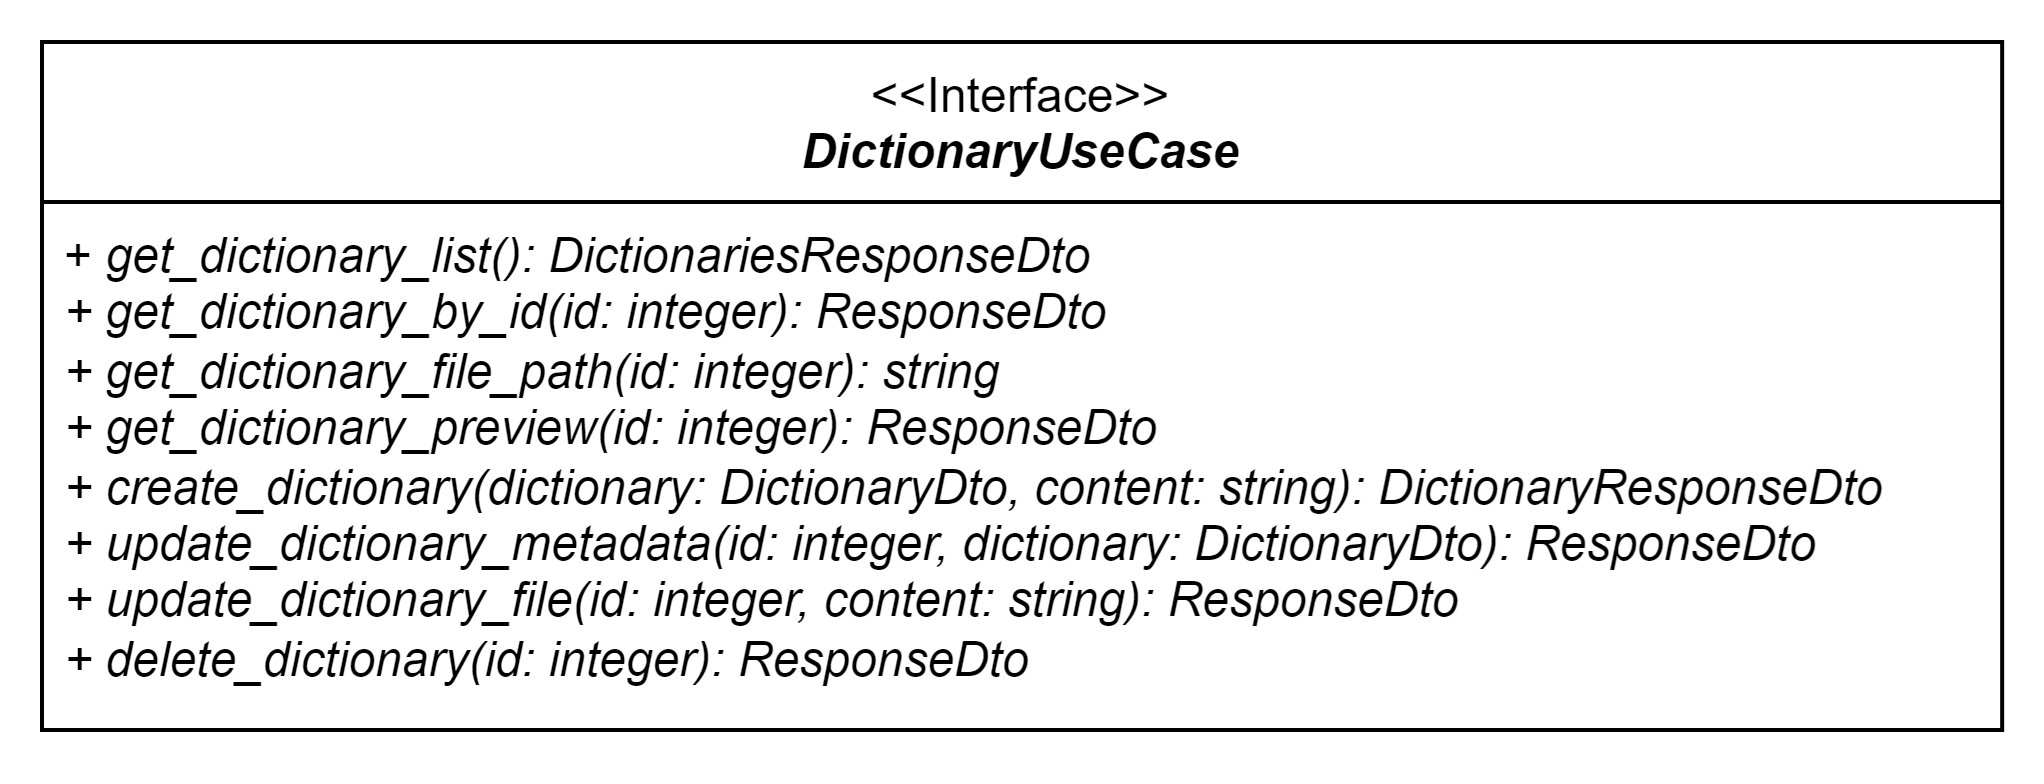
\includegraphics[width=0.75\textwidth]{assets/Backend/dictionary_use_case.png}
    \caption{Diagramma dell'interfaccia DictionaryUseCase}
  \end{figure}
\begin{itemize}
    \item \textbf{Descrizione}: DictionaryUseCase definisce il contratto per i casi d'uso relativi alla gestione dei \glossario{dizionari dati};
    \item \textbf{Operazioni}:
    \begin{itemize}
      \item Recupero delle informazioni di tutti i dizionari;
      \item Recupero delle informazioni di un dizionario;
      \item Recupero del percorso del file di un dizionario;
      \item Anteprima di un dizionario;
      \item Creazione di un dizionario;
      \item Aggiornamento dei metadati di un dizionario;
      \item Aggiornamento del file di un dizionario;
      \item Eliminazione di un dizionario.
    \end{itemize}
    \item \textbf{Implementazione}: i dettagli dell'implementazione sono riportati nelle classi concrete.
\end{itemize}  

\subsubsubsection{PromptUseCase} \label{PromptUseCase}
\begin{figure}[H]
    \centering
    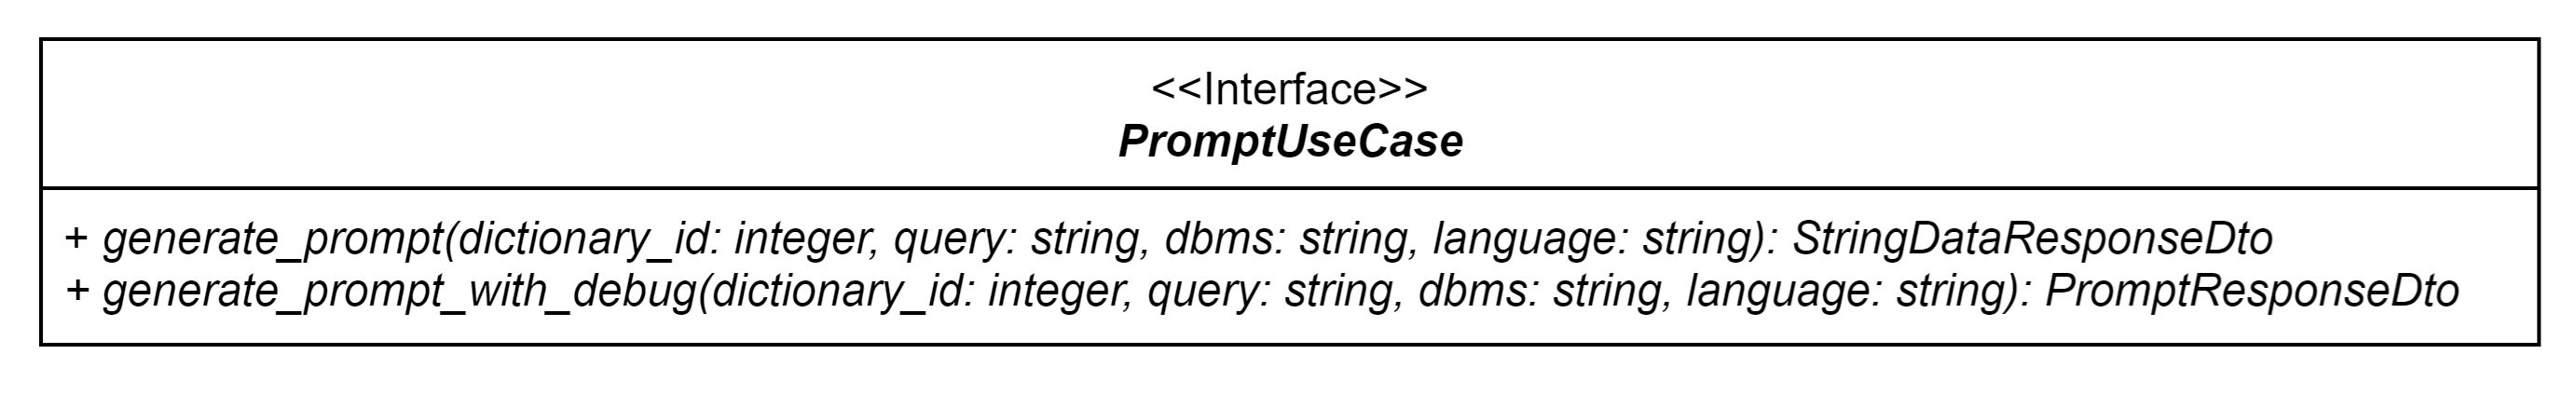
\includegraphics[width=0.9\textwidth]{assets/Backend/prompt_use_case.png}
    \caption{Diagramma dell'interfaccia PromptUseCase}
  \end{figure}
\begin{itemize}
    \item \textbf{Descrizione}: PromptUseCase definisce il contratto per i casi d'uso relativi alla generazione del \glossario{prompt};
    \item \textbf{Operazioni}:
    \begin{itemize}
      \item Generazione del prompt a partire da una richiesta, un dizionario, una lingua e un \glossario{DBMS};
      \item Generazione del prompt con informazioni di debug associate ad esso.
    \end{itemize}
    \item \textbf{Implementazione}: i dettagli dell'implementazione sono riportati nelle classi concrete.
\end{itemize}  

\subsubsubsection{SchemaValidatorUseCase} \label{SchemaValidatorUseCase}
\begin{figure}[H]
    \centering
    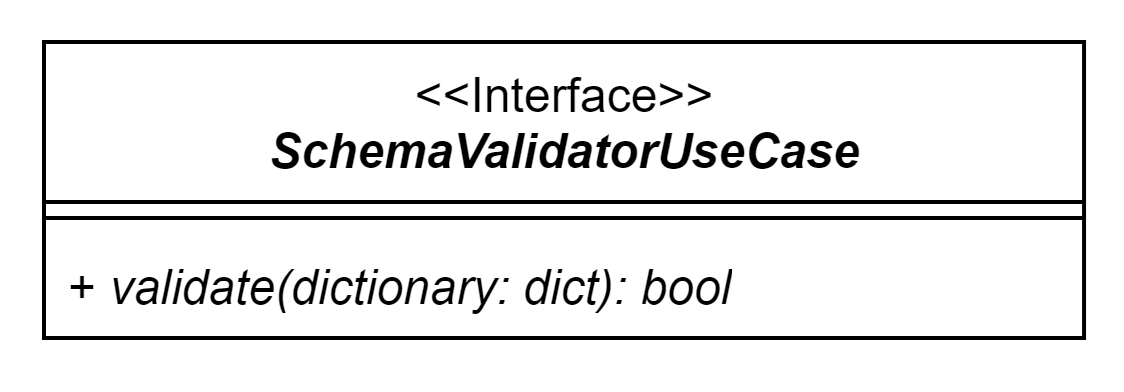
\includegraphics[width=0.6\textwidth]{assets/Backend/schema_validator_use_case.png}
    \caption{Diagramma dell'interfaccia SchemaValidatorUseCase}
  \end{figure}
\begin{itemize}
    \item \textbf{Descrizione}: SchemaValidatorUseCase definisce il contratto per i casi d'uso relativi alla validazione dello schema dei \glossario{dizionari dati};
    \item \textbf{Operazioni}:
    \begin{itemize}
      \item Validazione dello schema di un dizionario dati.
    \end{itemize}
    \item \textbf{Implementazione}: i dettagli dell'implementazione sono riportati nelle classi concrete.
\end{itemize}  

\subsubsubsection{Ports - Outcoming}

\subsubsubsection{EmbeddingsAbstractFactory} \label{EmbeddingsAbstractFactory}
\begin{figure}[H]
    \centering
    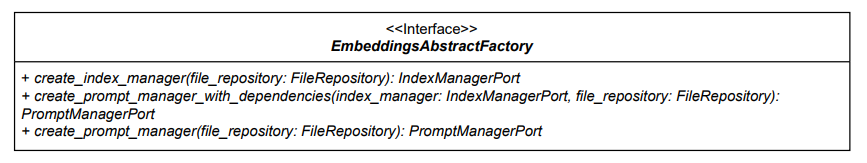
\includegraphics[width=0.8\textwidth]{assets/Backend/embeddings_abstract_factory.png}
    \caption{Diagramma dell'interfaccia EmbeddingsAbstractFactory}
  \end{figure}
\begin{itemize}
    \item \textbf{Descrizione}: EmbeddingsAbstractFactory fornisce una struttura per la creazione dei componenti relativi agli \glossario{embeddings} e alla generazione di \glossario{prompt};
    \item \textbf{Operazioni}:
    \begin{itemize}
      \item Creazione di un'istanza del gestore degli \glossario{indici};
      \item Creazione di un'istanza del gestore dei prompt.
    \end{itemize}
    \item \textbf{Implementazione}: i dettagli dell'implementazione sono riportati nelle classi concrete;
    \item \textbf{Dipendenze}:
    \begin{itemize}
        \item FileRepository;
        \item IndexManagerPort;
        \item PromptManagerPort.
    \end{itemize}
\end{itemize}  

\subsubsubsection{IndexManagerPort} \label{IndexManagerPort}
\begin{figure}[H]
    \centering
    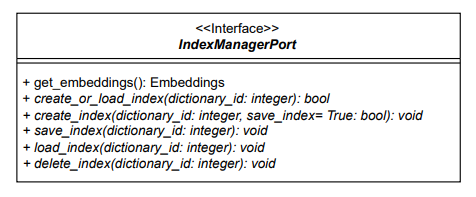
\includegraphics[width=0.7\textwidth]{assets/Backend/index_manager_port.png}
    \caption{Diagramma dell'interfaccia IndexManagerPort}
  \end{figure}
\begin{itemize}
    \item \textbf{Descrizione}: IndexManagerPort fornisce un'interfaccia per gestire le operazioni \glossario{CRUD} relative agli \glossario{embeddings};
    \item \textbf{Operazioni}:
    \begin{itemize}
      \item Recupero degli embeddings;
      \item Creazione di un \glossario{indice};
      \item Salvataggio di un indice;
      \item Ripristino di un indice;
      \item Eliminazione di un indice.
    \end{itemize}
    \item \textbf{Implementazione}: i dettagli dell'implementazione sono riportati nelle classi concrete.
\end{itemize} 

\subsubsubsection{PromptManagerPort} \label{PromptManagerPort}
\begin{figure}[H]
    \centering
    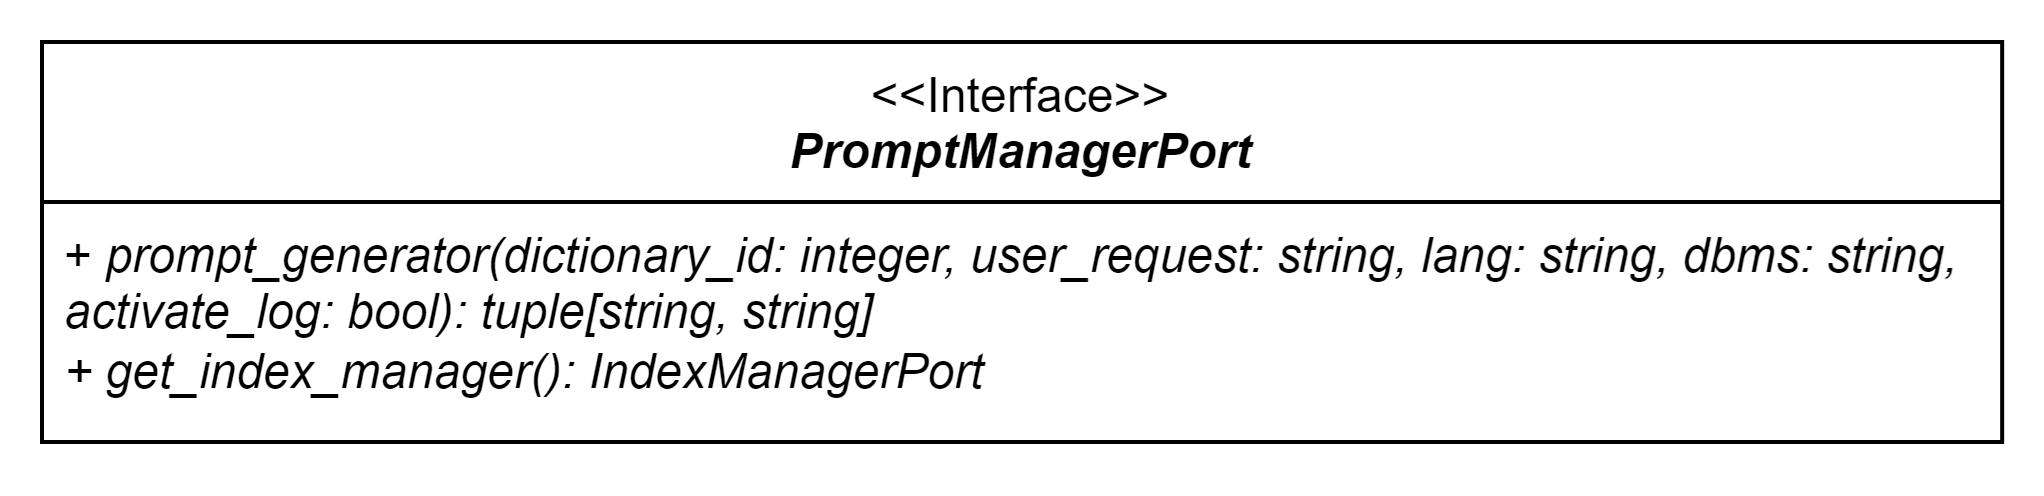
\includegraphics[width=0.7\textwidth]{assets/Backend/prompt_manager_port.png}
    \caption{Diagramma dell'interfaccia PromptManagerPort}
  \end{figure}
\begin{itemize}
    \item \textbf{Descrizione}: PromptManagerPort definisce il contratto per la generazione di \glossario{prompt};
    \item \textbf{Operazioni}:
    \begin{itemize}
      \item Generazione del prompt;
      \item Recupero dell'istanza del gestore degli \glossario{indici};
      \item Creazione dell'istanza del gestore di \glossario{debug}.
    \end{itemize}
    \item \textbf{Implementazione}: i dettagli dell'implementazione sono riportati nelle classi concrete;
    \item \textbf{Dipendenze}:
    \begin{itemize}
        \item IndexManagerPort;
        \item DebugManagerPort.
    \end{itemize}
\end{itemize} 

\subsubsubsection{DebugManagerPort} \label{DebugManagerPort}
\begin{figure}[H]
    \centering
    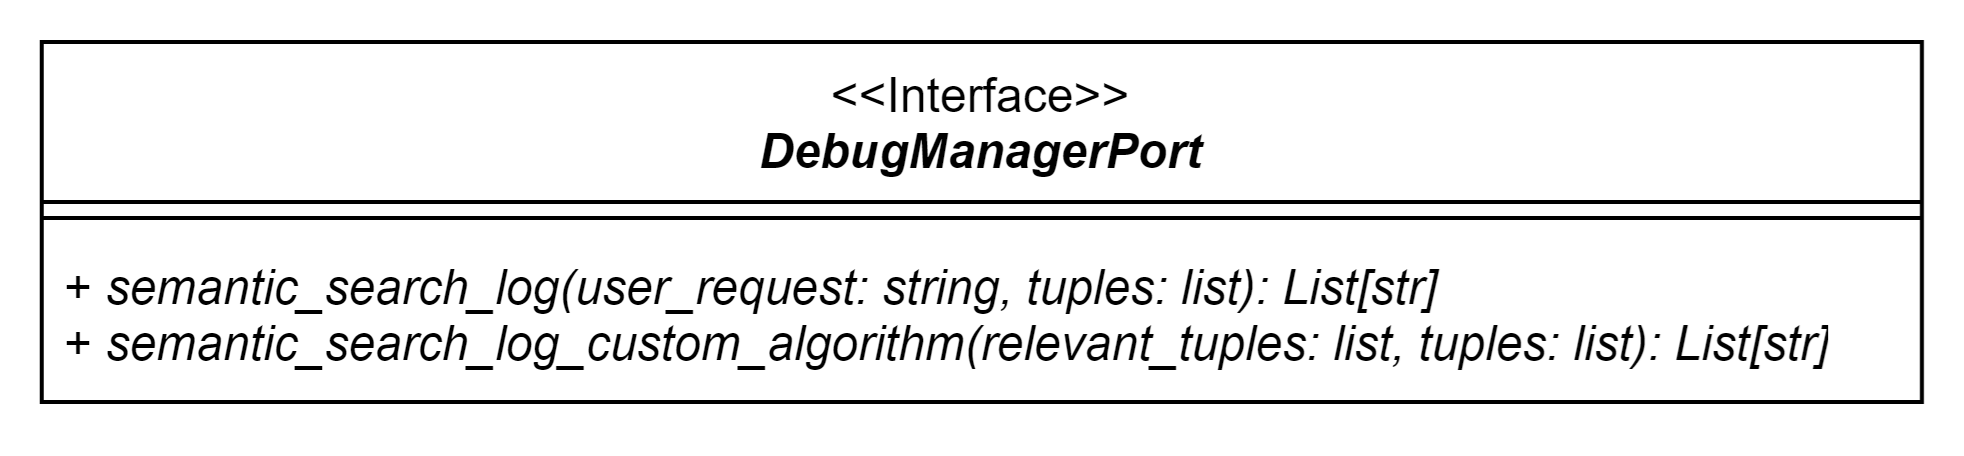
\includegraphics[width=0.7\textwidth]{assets/Backend/debug_manager_port.png}
    \caption{Diagramma dell'interfaccia DebugManagerPort}
  \end{figure}
\begin{itemize}
    \item \textbf{Descrizione}: DebugManagerPort definisce il contratto per la gestione dei \glossario{log} relativi alle operazioni di ricerca semantica;
    \item \textbf{Operazioni}:
    \begin{itemize}
      \item \glossario{Debug} di un'operazione di ricerca semantica.
    \end{itemize}
    \item \textbf{Implementazione}: i dettagli dell'implementazione sono riportati nelle classi concrete.
\end{itemize}  

\subsubsubsection{DbManagerAbstractFactory} \label{DbManagerAbstractFactory}
\begin{figure}[H]
    \centering
    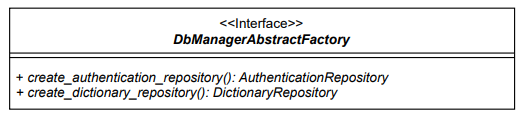
\includegraphics[width=0.7\textwidth]{assets/Backend/db_manager_abstract_factory.png}
    \caption{Diagramma dell'interfaccia DbManagerAbstractFactory}
  \end{figure}
\begin{itemize}
    \item \textbf{Descrizione}: DbManagerAbstractFactory fornisce una struttura per la creazione dei componenti relativi alla gestione dei dizionari e degli utenti;
    \item \textbf{Operazioni}:
    \begin{itemize}
      \item Creazione di un'istanza della classe per la gestione degli utenti;
      \item Creazione di un'istanza della classe per la gestione dei dizionari.
    \end{itemize}
    \item \textbf{Implementazione}: i dettagli dell'implementazione sono riportati nelle classi concrete;
    \item \textbf{Dipendenze}:
    \begin{itemize}
      \item AuthenticationRepository;
      \item DictionaryRepository.
    \end{itemize}
\end{itemize} 

\subsubsubsection{AuthenticationRepository} \label{AuthenticationRepository}
\begin{figure}[H]
    \centering
    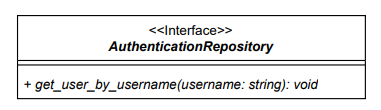
\includegraphics[width=0.65\textwidth]{assets/Backend/authentication_repository.png}
    \caption{Diagramma dell'interfaccia AuthenticationRepository}
  \end{figure}
\begin{itemize}
    \item \textbf{Descrizione}: AuthenticationRepository definisce un contratto per l'accesso e la gestione dei dati di autenticazione degli utenti;
    \item \textbf{Operazioni}: 
    \begin{itemize}
      \item Recupera i dettagli di un utente tramite lo username.
    \end{itemize}
    \item \textbf{Implementazione}: i dettagli dell'implementazione sono riportati nelle classi concrete.
\end{itemize}

\subsubsubsection{DictionaryRepository} \label{DictionaryRepository}
\begin{figure}[H]
    \centering
    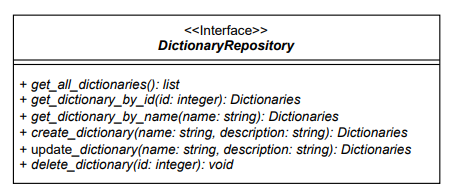
\includegraphics[width=0.7\textwidth]{assets/Backend/dictionary_repository.png}
    \caption{Diagramma dell'interfaccia DictionaryRepository}
  \end{figure}
\begin{itemize}
  \item \textbf{Descrizione}: DictionaryRepository definisce un contratto per la gestione dei dizionari all'interno del sistema; 
  \item \textbf{Operazioni}: 
    \begin{itemize}
      \item Recupero delle informazioni di tutti i dizionari;
      \item Recupero delle informazioni di un dizionario tramite il suo ID;
      \item Recupero delle informazioni di un dizionario tramite il suo nome;
      \item Creazione di un dizionario;
      \item Aggiornamento dei metadati di un dizionario;
      \item Eliminazione di un dizionario.
    \end{itemize}
  \item \textbf{Implementazione}: i dettagli dell'implementazione sono riportati nelle classi concrete.
\end{itemize} 

\subsubsubsection{FileRepository} \label{FileRepository}
\begin{figure}[H]
    \centering
    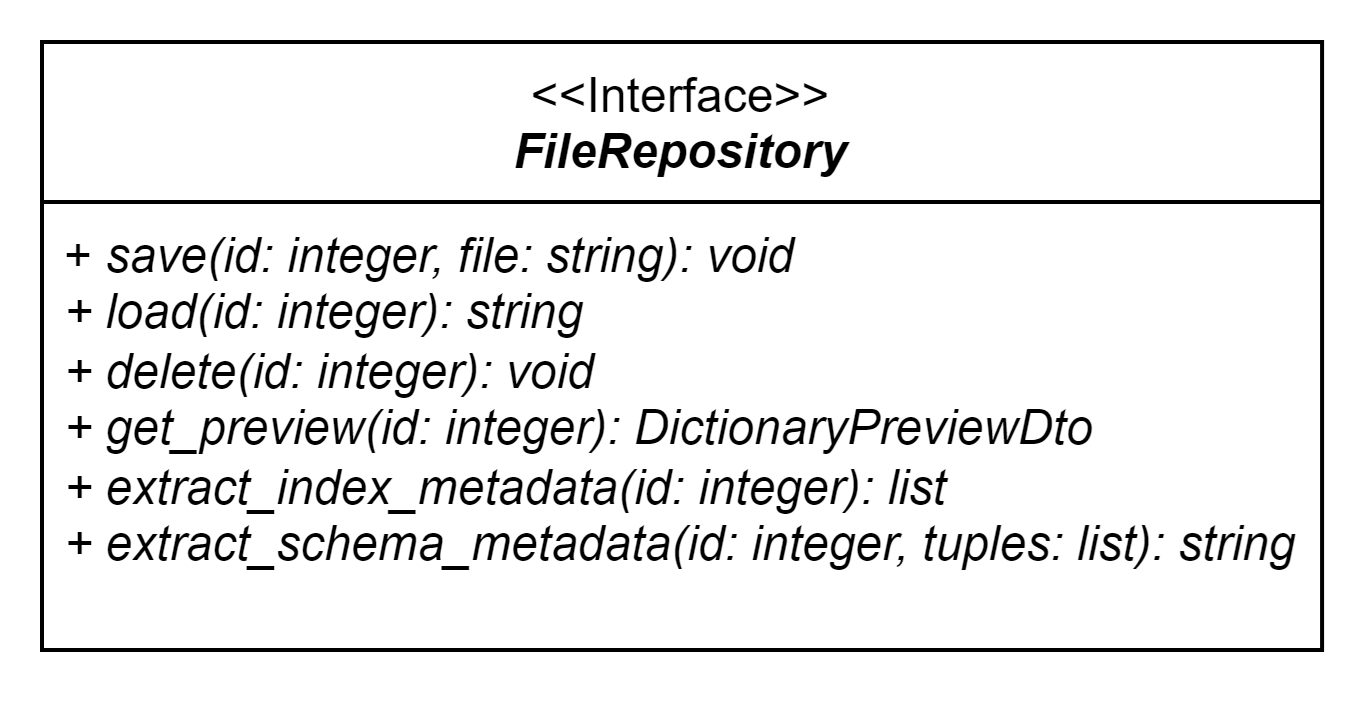
\includegraphics[width=0.65\textwidth]{assets/Backend/file_repository.png}
    \caption{Diagramma dell'interfaccia FileRepository}
  \end{figure}
\begin{itemize}
  \item \textbf{Descrizione}: FileRepository definisce un contratto per la gestione delle operazioni \glossario{CRUD} sui file associati ai dizionari;
  \item \textbf{Operazioni}: 
    \begin{itemize}
      \item Salvataggio di un file;
      \item Recupero del percorso di un file;
      \item Eliminazione di un file;
      \item Estrazione di un'anteprima del contenuto di un file;
      \item Estrazione dei metadati di un file per l'\glossario{indicizzazione};
      \item Estrazione dei metadati di un file in forma di \glossario{prompt}.
    \end{itemize}
  \item \textbf{Implementazione}: i dettagli dell'implementazione sono riportati nelle classi concrete.
\end{itemize} 